 \documentclass{sig-alternate}
 
 \begin{document}

% In the original styles from ACM, you would have needed to
% add meta-info here. This is not necessary for AAMAS 2012  as
% the complete copyright information is generated by the cls-files.
  \conferenceinfo{GECCO'13,} {July 6-10, 2013, Amsterdam, The Netherlands.}
    \CopyrightYear{2013}
    \crdata{TBA}
    \clubpenalty=10000
    \widowpenalty = 10000
%Overall TODOS: 
%Remove all mention of Q learning or action value.
%Remove all mention of aircraft being agents and replace them with gates being agents.
%Fix global and system-level reward. "system-level, or global reward, is..."
%Replace Figures 4 5 and 6
%Fix Grammar errors
%Replace difference reward to difference evaluation function, global reward with global fitness, reward shaping with fitness function shaping, reinforcement learning with evolutionary algorithm

%Separation, etc. has been applied in other work, we chose to use en route delay to demonstrate partitioning and learning in difficult problems with hard constraints.

%The agents are rewarded based on their original actions. Greedy scheduler is stochastic, and therefore a policy converged agent is able to predict what the greedy scheduler will do to its initial action.

%We use basic agglomerative hierarchical clustering where the closest two clusters are merged together. We let this algorithm run for some amount of time and obtain many different cluster sizes.

%Centralized pre-processing clustering. Future work section: Automated decentralized and centralized clustering based on no prior knowledge of the system.


\title{Partitioning Agents and Shaping Their Evaluation Functions in Air Traffic Problems with Hard Constraints}

\numberofauthors{3}

\author{
% You can go ahead and credit any number of authors here,
% e.g. one 'row of three' or two rows (consisting of one row of three
% and a second row of one, two or three).
%
% The command \alignauthor (no curly braces needed) should
% precede each author name, affiliation/snail-mail address and
% e-mail address. Additionally, tag each line of
% affiliation/address with \affaddr, and tag the
% e-mail address with \email.
% 1st. author
\alignauthor
%William Curran\\
%       \affaddr{Oregon State University}\\
%       \affaddr{Address}\\
%      \affaddr{Corvallis, Oregon}\\
%       \email{curranw@onid.orst.edu}
% 2nd. author
%\alignauthor
%Adrian Agogino\\
%       \affaddr{NASA Ames Research Center}\\
%       \affaddr{Address}\\
%       \affaddr{Moffet Field, California}\\
%       \email{adrian.k.agogino@nasa.gov}
% 3rd. author
%\alignauthor 
%Kagan Tumer\\
%       \affaddr{Oregon State University}\\
%       \affaddr{Address}\\
%       \affaddr{Corvallis, Oregon}\\
%       \email{kagan.tumer@oregonstate.edu}
}


\maketitle
\begin{abstract}
Hundreds of thousands of hours of delay, costing millions of dollars annually, are reported by airports in the US alone. Weather and airport conditions may instigate this delay, but routing decisions balancing delay with congestion contribute significantly to the propagation of delays throughout the US airspace. The task of managing delay may be seen as a multiagent congestion problem. In this problem there are many tightly coupled agents whose actions collectively impact the system, making it difficult for agents to learn how they impact the system. Fitness function shaping is effective at improving agent learning for soft constraint problems by reducing learning noise caused by agent interactions, so we extend those results to hard constraints that cannot be easily learned, and must be enforced algorithmically. We present an agent partitioning algorithm in conjunction with fitness function shaping to simplify the learning domain. Our results show that an autonomous partitioning of the agents using system features leads to up to 30x speed over simple hard constraint enforcement, as well as up to a 21\% improvement in performance over a greedy scheduling solution corresponding to hundreds of hours of delay saved in a single day.
\end{abstract}


\category{I.2.11}{Distributed Artificial Intelligence}{Multiagent systems}

\terms{Algorithms}

\keywords{Aerospace Industry, Multiagent systems}

\vspace{100pt}
\section{Introduction}
A primary concern facing the aerospace industry today is the efficient, safe and reliable management of our ever-increasing air traffic. In 2011, weather, routing decisions and airport conditions caused 330,063 delays, accounting for 266,999 hours of delay \cite{faa05}. Many of these delays in the National Airspace System (NAS) are caused by en route, landing, or departing airspace congestion. The increase in flights being scheduled is much faster than that of airports being built, making effective traffic control algorithms essential. We refer to the task of managing delay in the system by coordinating aircraft as the Air Traffic Flow Management Problem (ATFMP). 

Typical methods to alleviate delay in the ATFMP involve imposing ground delay on aircraft, changing the speed of en route aircraft, and changing separation between aircraft. Because the airspace has many connections from one airport to another, the congestion and associated delay can propagate throughout the system. Delays may be imposed to better coordinate aircraft and mitigate the propagation of congestion and the associated delay, but which aircraft should be delayed? The search space in such a problem is huge, as there are tens of thousands of flights every day within the United States.

Current approaches to the ATFMP include the use of binary integer programming \cite{Bertsimas}, evolutionary approaches \cite{Rios}, and multiagent reinforcement learning \cite{tumer-agogino_jaamas12}. The most recent complete overview of the ATFMP in practice is provided by Sridhar, Grabbe, and Mukherjee \cite{Sridhar}. These approaches reduce delay in the NAS, but either have not been expanded to an entire 24 hours aircraft data or does not completely remove all congestion from the system. 

We propose an approach to solving the problem that blends multiagent coordination, fitness function shaping, automated agent partitioning, and hard constraint optimization. Multiagent coordination and fitness function shaping give us the ability to perform an intelligent guided search over tens of thousands of aircraft actions, while the hard constraint allows us to completely remove congestion. In the ATFMP, multiagent coordination with fitness function shaping becomes a computationally intractable task, therefore we used automated agent partitioning to reduce the overhead associated with the hard constraint. 

The remainder of this paper is organized as follows. Section 2 describes the related work in the ATFMP, constraint optimization, multiagent coordination, and fitness function shaping. In Section 3 we describe the experimental approach taken using multiagent coordination, the difference evaluation function, the greedy scheduler and agent partitioning. Experimental results are then provided in Section 4, followed by the conclusion and future work in Section 5.

\section{Related Work}
To motivate our approach, we introduce the fitness function shaping technique known as the difference evaluation function, hard constraint optimization, and a brief description and overview of the previous work done in the ATFMP.
  
\subsection{Air Traffic Flow Management}
The ATFMP addresses the congestion in the NAS by controlling ground delay, en route speed or changing separation between aircraft. The NAS is divided into many sectors, each with a restriction on the number of aircraft that may fly through it at a given time. This number is formulated by the FAA and is calculated from the number of air traffic controllers in the sector, the weather, and the geographic location. These sector capacities are known as en route capacities. Additionally, each airport in the NAS has an arrival and departure capacity that cannot be exceeded. Eliminating the congestion in the system while keeping the amount of delay each aircraft incurs small is the fundamental goal of ATFMP. 

Previous work in the ATFMP had applied Integer Linear Programming \cite{Bertsimas}, evolutionary approaches \cite{Rios}, and multiagent approaches \cite{tumer-agogino_jaamas12,664154, Sislak:2008:AMA:1402744.1402755}. The ATFMP is a naturally distributed problem with complex interactions among all aircraft and airports. This renders pre-determined centralized solutions to become suboptimal whenever there is any derivation from the expected air traffic flow. Therefore using a decentralized multiagent system is an ideal approach in such a domain.

There are three main issues to using Integer Linear Programming (IPLP) that are removed using a multiagent approach; first, designing an IPLP algorithm for a particular task is a difficult process, and it takes a lot of effort to adapt IPLP to new problem variations that inevitably come up. Second, formulation of IPLP is complex even for simple problems. For real world implementations there are likely to be an enormous amount of subtle complexity that has to be included in the system, such as balancing the needs to airlines, air traffic controllers and passengers. These complexities can be added in a straight forward way in fitness evaluation functions, but not in IPLP. Third is computational complexity; IPLP computation can grow exponentially with problem size. A carefully designed IPLP can avoid this exponential increase within a certain range of parameters, but after a certain problem size, computing an IPLP solution is infeasible.

\subsection{Constraint Optimization}

Typical learning algorithms use soft constraint optimization and attempt to minimize all objectives in the system. These are usually formulated as a multi-objective learning problem where agents receive a reward or fitness that is some combination of all objectives. Hard constraint optimization on the other hand can assist multiagent coordination by forcing a constraint to be satisfied, and attempting to optimize the rest of the reward. This approach simplifies a more complicated multi-objective coordination problem into a more simple single-objective problem.

One approach to constraint optimization is Distributed Constraint Optimization (DCOP) \cite{Junges:2008:EPD:1402298.1402308, Modi:2005:AAD:1120120.1120127}. DCOPs are well-suited for modeling multiagent coordination problems with many interactions between agents. We used multiagent evolutionary algorithms because of the large number of agents and intend to extend the scope of our experiments to include uncertainty in future work.

Greedy search algorithms, such as a greedy scheduler, can enforce hard constraints by forcing one of the objectives to zero while sacrificing the other objectives. Previous approaches to the ATFMP use a greedy heuristic scheduler \cite{Rios} to enforce congestion constraints. The greedy scheduler checks to see if a plane's flight plan causes any sectors to become congested. If the plane causes congestion, it is delayed by one minute, and then the congestion is recalculated. This adds delay by completely removing congestion out of the system. The greedy scheduler is necessary in this domain to accomplish this congestion removal. This is a necessity of the problem: congestion in this domain means that there is not enough air traffic control personnel to handle the traffic, and is therefore dangerous.

Due to the heuristic nature of the scheduler, it is suboptimal and a guided search must be performed to improve performance. This solution requires a learning algorithm to first choose actions for the agents, then have those actions modified by the greedy scheduler, and finally give feedback to the learning algorithm based upon the system after the greedy scheduler and the original actions taken.

%When combining hard constraint optimization and the benefits of the difference reward, there are computational issues. In order to compute the difference reward, the greedy scheduler must be ran for each aircraft in order to analyze the amount of impact the aircraft had on the system. This, by itself, is a computationally intractable problem. We deal with this by autonomously partitioning agents using pre-processed features about each agent. An agent partition consists of agents that impact each other more than other aircraft, therefore the reward can be calculated relative to only those aircraft. The greedy scheduler can then schedule only aircraft within a partition, keeping all other aircraft static. This vastly reduces the amount of computation needed to run the greedy scheduler, and makes this approach feasible. 

\subsection{Fitness Function Shaping for coordination}
Multiagent coordination is an important aspect of many domains, such as data routing \cite{tumer-wolpert_jair02}, air traffic control \cite{tumer-agogino_jaamas12, Sislak:2008:AMA:1402744.1402755}, Robocup soccer \cite{AAMAS12-agmon} and multi-robot coordination \cite{5509316}. Most multiagent coordination problems cannot use typical search algorithms, such as breadth first search or A* search, due to the combinatorial search space increase and lack of coordination. A learning or evolutionary algorithm will often convert a once computationally intractable search problem into a feasible guided search. 

In evolutionary algorithms fitness function design is important in keeping convergence time low, while keeping policy performance high. In many multiagent coordination domains there is the discrepancy between maximizing the system-level evaluation and maximizing a single agent's evaluation. If an agent always greedily takes the locally optimal action, it does not always maximize the system-level evaluation; this is known as the Tragedy of the Commons \cite{Hardin}.

The difference evaluation function \cite{tumer-wolpert_jair02} is evaluated such that each agent's fitness is related to the individual's contribution to team performance, therefore the signal-to-noise ratio is improved considerably. This leads to final better policies at an accelerated converge rate, as well as overcoming the Tragedy of the Commons. The difference evaluation function is defined as:

\begin{equation}
D_i(z) = G(z) - G(z - z_i + c)\;,
\end{equation}

where \textit{z} is the system state, $z_i$ is the system state with agent $i$, and $c$ is a counterfactual replacing agent $i$. This counterfactual offsets the artificial impact of removing an agent from the system. For example, removing an aircraft from the system always artificially decreases the amount of congestion and delay, which would provide a poor evaluation if a counterfactual is not used.

The difference evaluation function provides a compact encapsulation of the agents impact on the system. A domain with many agents as well as highly coupled actions suffers when using fitnesses such as the system-level (global) evaluation or local evaluation. System-level evaluations allow an agent to identify whether the joint action of all the agents increases the system's performance, but cannot determine whether its own action produces the increase or if another agent was responsible. This leads to a very noisy evaluation. Local evaluations can always identify whether an action had some positive or negative effects, but these local evaluations do not overcome the Tragedy of the Commons. In highly coupled domains local evaluations severely hurts system-level performance, while the sheer number of agents cause agents to learn very slowly from system-level evaluations due to the noise, these system-level evaluations tend to also converge to suboptimal policies. The difference evaluation reduces the noise from other agents in the evaluation and has proven to outperform both system-level and local evaluations in many congestion domains \cite{tumer-agogino_jaamas08, tumer-wolpert_jair02}.

In many systems it is difficult or impossible to calculate the difference evaluation without resimulation, which can become prohibitively costly. If resimulation is highly optimized, or the difference evaluation function is easily approximated, this evaluation function is a powerful tool for multiagent coordination.

\section{Approach to Hard Constraint Optimization}

Our approach to traffic flow management involved five main concepts: formulating a multiagent congestion problem by defining agents, formulating the appropriate system fitness function and fitness function shaping, blending the heuristic greedy scheduler with multiagent evolution, and performing hard constraint optimization through the use of agent partitioning.

\subsection{Agent Definition}
There are many possible definitions for an agent in this domain. In this paper, agents were assigned to aircraft terminals, emphasizing the cooperative nature of the scheduling. There is one airport terminal representing each aircraft. This decentralized solution benefits from many advantages. One of which is that each aircraft has its own policy, eliminating the need for a centralized controller. Another is that agents can be easily partitioned into independent groups, simplifying the learning problem.  

Agents have no state, but may select a certain amount of ground delay from 0 to 10 minutes (11 actions) in the beginning of every simulation. The agent does not have the capability to change their action based upon the system state once the simulation starts, therefore feedback can only be given once per simulation.

\subsection{Agent Evolution}
Agents evolved using traditional cooperative coevolutionary algorithms (CCEAs). In CCEAs, fitnesses assigned to population members are based on the interactions with the population members in a given team. Each population member is randomly assigned with population members of other agents to create a team. This team is evaluated and each population member is given a fitness. Once all population members have been assigned to a team, evolutionary subsampling is performed. For this evolutionary algorithm, we use 10 population members per agent with a mutation rate of 10\%, and zero crossover. 

CCEAs are well suited for multiagent domains where robustness is a desirable quality, and agents need to succeed, or fail, as a team. The random population member assignment generates a robustness well suited for the ATFMP, as a solution needs to be able to withstand sudden schedule changes that are frequent in air traffic, such as weather delays. Although robustness is nice, the key advantage of this approach is each agent only has to search a subspace of the entire state space. Without this reduced state space, convergence is not possible in the ATFMP. 

\subsection{Fitness Evaluation}
The system-level evaluation we developed focuses on the cumulative delay ($\delta$) and congestion ($C$) throughout the system:

\begin{equation}
G(z) = -(C(z)^w + \delta(z))\;,
\end{equation}

where \textit{C(z)} is the total congestion penalty and \textit{$\delta$(z)} is the cumulative system delay. The importance of congestion over delay is represented by the weight \textit{w}. Although minimizing delay is important, minimizing congestion is required for safety within the NAS. Therefore, minimizing delay must be performed simultaneously to minimizing congestion to zero, meaning the weight for congestion must be higher than delay.

The total delay is the sum of delays over all aircraft. This is a linear combination of the amount of ground delay and the amount of scheduler delay an agent incurred:

\begin{equation}
\delta(z) = \displaystyle\sum\limits_{a \in A} \delta_{g,a}(z) + \delta_{s,a}(z)\;,
\end{equation}

where $\delta_{g,a}(z)$ is the ground delay the aircraft incurred and $\delta_{s,a}(z)$ is the scheduler delay the aircraft incurred. 

The total congestion penalty is the sum of differences between sector capacity and the current sector congestion:

\begin{equation}
C(z) = \displaystyle\sum\limits_{s \in S} C_s(z)\;,
\end{equation}

where

\begin{equation}
C_s(z) = \displaystyle\sum\limits_{t \in T} \theta(C_{t,s} - S_s) (C_{t,s} - S_s)\;,
\end{equation}

where $S_s$ is the sector capacity of sector s as defined by the FAA and $\theta$ is a step function that equals 1 if its argument is greater than 0, and 0 otherwise. In this way, agents are penalized when a sector exceeds its capacity.

Minimizing congestion involves intelligently adding ground delay to specific aircraft to obtain smallest amount of system congestion possible. In this problem, removing congestion from the system adds delay, and removing delay from the system could potentially add congestion, and as you can see in Figure \ref{delayCongestionPower} this is not a 1:1 mapping. Removing a little congestion from the system still requires the introduction of quite a bit of delay. Minimizing this cost to delay for every reduction in congestion is important to a stable solution.

With so many agents, tens of thousands of actions simultaneously impact the system, causing the fitness for a specific agent to become noisy with the actions of other agents. An agent would have difficulty evolving to an optimal solution using such a noisy fitness evaluation signal. A difference evaluation function reduces much of this noise, and is easily derived from the system-level evaluation function:

\begin{equation}
D(z) = C^w(z-z_j + c_j) - C^w + \delta(z-z_j + c_j) - \delta\;,
\end{equation}

where \textit{$\delta(z-z_j + c_j)$} and \textit{$C(z-z_j + c_j)$} are the cumulative delay and congestion of all agents with agent $j$ replaced with counterfactual \textit{$c_j$}. We used a non-zero counterfactual for two reasons. One, if you remove an aircraft from the system, the fitness evaluation given to the agents is artificially increased. Furthermore, the aircraft are less likely to cause conflicts due to the easier scheduling problem. Two, we used a counterfactual where the agent does not delay at all, meaning that if not delaying produces a higher fitness evaluation than delaying, this policy should be found quickly. We also take advantage of the fact that most airplanes do not need to be delayed. If the counterfactual is equal to the agent, the difference evaluation function becomes zero and does not need to be calculated, thus speeding up fitness assignment.

\subsection{Heuristic Approaches}
We first converted the multi-objective problem to a single-objective problem by increasing the exponential weight \textit{w} on the total congestion, as used in equation 4. As \textit{w} increases, the delay impact on the system becomes negligible. Thus the agent will begin ignoring the delay and only attempt to optimize congestion. This turned the multi-objective problem into a single-objective problem, but still kept sector congestion as a soft constraint.

Preliminary results, shown in Figure \ref{delayCongestionPower} indicate that this is an impractical solution. With a weight of 1, the congestion and delay are equally optimized, leading to a balanced solution. When the weight on congestion increases to two or higher, the congestion converges to the same suboptimal point at different speeds. The agent will never evolve to an optimal policy that decreases congestion at the cost of delay, no matter how much emphasis is placed on congestion. Using exponential weights to convert this multi-objective problem to a single-objective problem does not work.

\begin{figure}[tbh!]
\centering
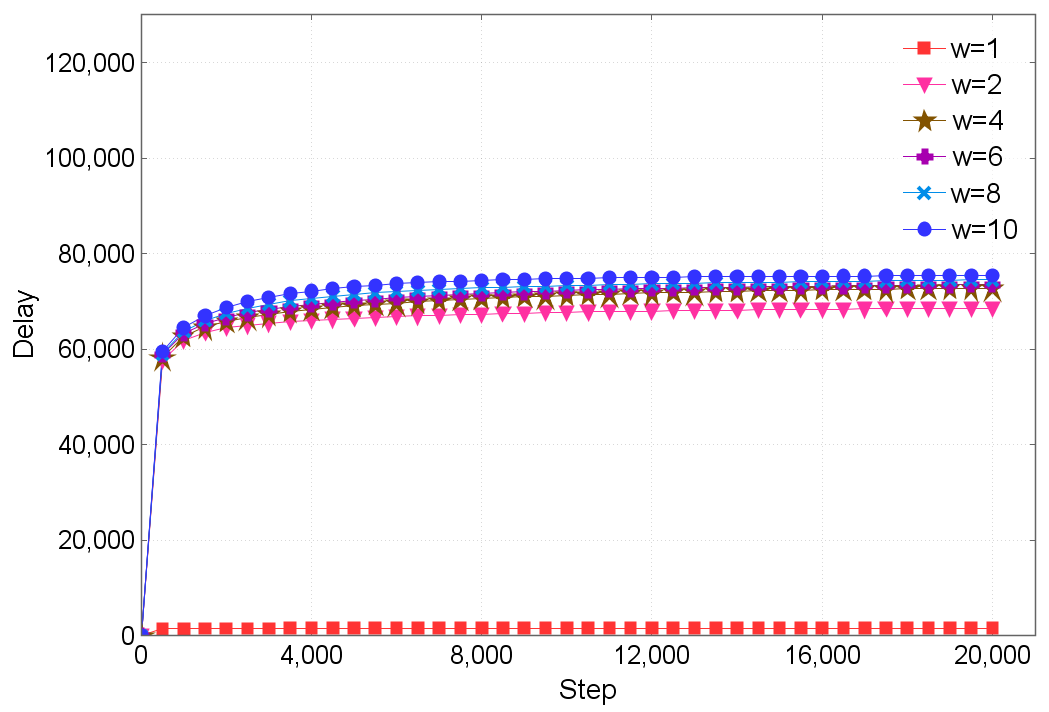
\includegraphics[width=1.0\columnwidth]{delayPower}
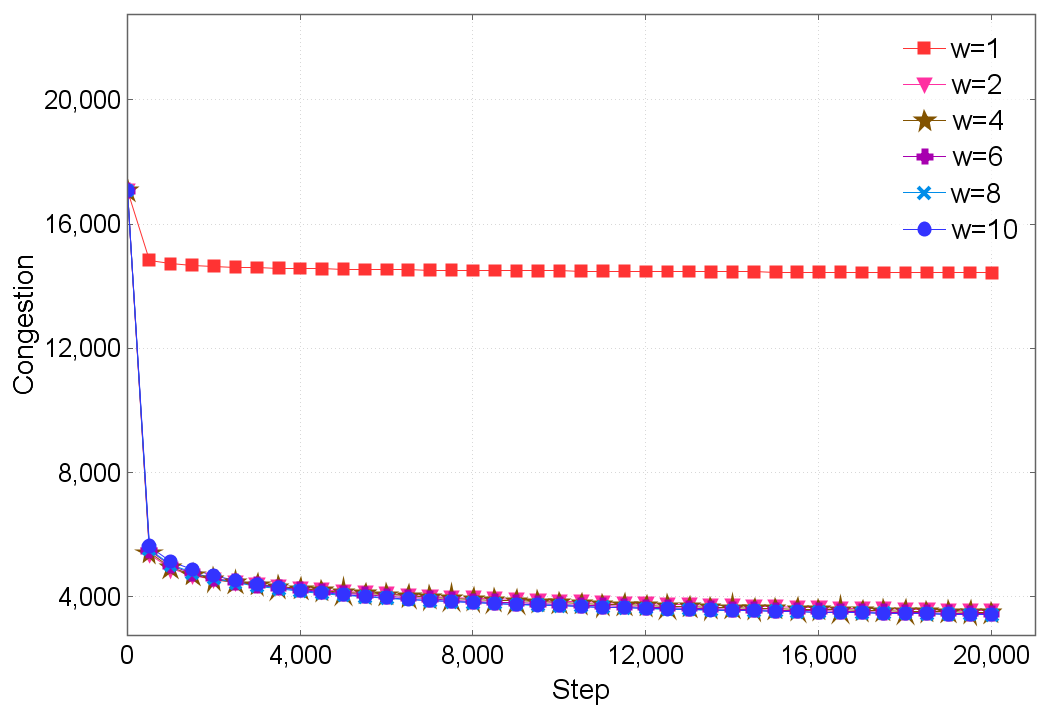
\includegraphics[width=1.0\columnwidth]{congestionPower}
\caption{Delay and congestion with varying $w$, the weight on congestion. No matter the weight, the evolutionary algorithm will not remove congestion while attempting to keep delay low. Additionally the cost to delay for when removing congestion is not a 1:1 mapping. A removal of 10,000 congestion adds 70,000 minutes of delay}
\label{delayCongestionPower}
\end{figure}

To solve this problem we introduce a greedy scheduler. The greedy scheduler will convert sector congestion into a hard constraint, causing any amount of delay to achieve the goal. If any aircraft's flight plan violates the capacity constraint of any sector, it is forced to ground delay for 1 additional minute. Using the greedy scheduler forces congestion to become zero and therefore be taken out of the system utility.

Although the greedy scheduler is useful in removing congestion, it cannot optimize delay. A simple solution would be to make every aircraft have a ground delay of 0, and have the greedy scheduler fix any conflicts, but this does not work. Due to the congestion in the system, a delay of 0 for each aircraft would be suboptimal. The greedy scheduler will assign delay without taking into account agent coordination. CCEAs discovers a good ground delay for each aircraft, preventing the need to perform an exhaustive search.

\subsection{Hard Constraint Optimization}
The ATFMP has been previously analyzed using only a small time window. We wanted to approach this problem with a 14-hour window (28 hours from the first takeoff to the last landing aircraft). This dramatically increases the number of agents from thousands to 35,844. In this highly-congested coordination domain, it is difficult to achieve high performance without ensuring the agent's fitness evaluation fully encapsulates the impact it had on the system. 

The difference evaluation function was determined from the definition of the system-level evaluation function:

\begin{equation}
D(z) = (-\delta(z)) - (-\delta(z-z_j + c_j)))\;,
\end{equation}

where \textit{$\delta(z)$} is the cumulative delay in the system and \textit{$\delta(z-z_j + c_j)$} is the cumulative delay of with agent $j$ replaced with counterfactual \textit{$c_j$}.

This greedy scheduler can easily be combined with CCEAs (Figure \ref{LearningCycle}). A team of population members take an action, all actions are then modified using the greedy scheduler, reducing congestion to zero, and then each population member will be assigned a fitness based on the system after the greedy scheduler. When combining the difference evaluation with the greedy scheduler, there are severe computational issues. The difference evaluation requires an agent to be removed from the system, the greedy scheduler to reschedule all aircraft back into the system, and then compute the difference in delays. Rescheduling all 35,000 aircraft during each difference calculation makes this a computationally intractable solution. 

\begin{figure}[tbh!]
\centering
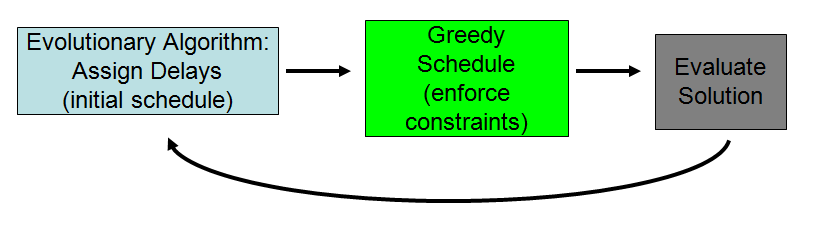
\includegraphics[width=.9\columnwidth]{LearningCycle}
\caption{Evaluation using the greedy scheduler}
\label{LearningCycle}
\end{figure}


\subsection{Agent Partitioning}
To reduce the computational overhead while computing the difference evaluation we reduced the number of aircraft the greedy scheduler had to reschedule by partitioning the aircraft into independent groups. The ATFMP has a clear partitioning of agents. Agents that do not go through the same sectors do not impact each other at all, and therefore can be treated as a smaller, more easily manageable, learning problem. 

One possible partitioning approach is to force every partition to be completely independent of every other partition. This requires a potential overlap of partitions, as typically many aircraft have partially or completely overlapping flight plans. Each partition is therefore a collection of overlapping flight plans with a small number of sectors unique to that partition. Although this approach achieves what we need, it typically results in one partition per aircraft and very large partitions. With 35,000 aircraft this approach becomes prohibitively computationally expensive.

Instead of the traditional approach, we applied agglomerative hierarchical clustering \cite{Agglomerative} to partition similar agents together. Each agent was partitioned with other agents based on the number of similar sectors they had within their flight plan. This was accomplished all during the pre-processing of the flight plan data. Partitioning reduces the number of aircraft into a more manageable size for learning, from 35,000 to on the order of hundreds or thousands.  The partitioning was stopped and saved at every iteration to obtain a varying size of partitions. 

When assigning a fitness to an agent, only the delay of the agents within their partition were taken into account. Therefore, the greedy scheduler only needs to schedule the size of the partition during each difference evaluation calculation. This dramatically reduces the time complexity and allows the difference evaluation to be efficiently combined with the greedy scheduler. This results in a new fitness for each partition $i$:

\begin{equation}
D_i(z) = (-\delta_i(z)) - (-\delta_i(z_i-z_{{i}_j} + c_j)))\;,
\end{equation}

where \textit{$\delta_i(z)$} is the cumulative delay of partition $i$ and \textit{$\delta_i(z_i-z_{{i}_j} + c_j)$} is the cumulative delay of partition $i$ with agent $j$ replaced with counterfactual \textit{$c_j$}.

\subsection{Simulator Characteristics}
We present a multiagent approach to traffic flow management based on agents taking independent actions that maximize a system utility. All agent's actions are then simulated in a simple traffic flow management simulator. This simulator needs only to store sector and time information for each flight and compute congestion for each sector. From the simulation we can compute congestion and ground delay in the system and assign fitnesses to population members accordingly.

Due to the simplicity of our simulation requirements, using complicated simulators such as FACET \cite{FACET} and AgentFly \cite{Sislak:2008:AMA:1402744.1402755} would cause many problems. We chose to create our own flight simulator for multiple reasons. First, the simulation is simple; the only requirement is to keep track of sector capacities per time step, given a list of flight planes. This is trivial to implement. Additionally, using CCEAs requires frequent of sampling from data, meaning that using more advanced simulators would result in an unnecessarily large time complexity.

\section{Experimental Results}
The experimental results in this paper analyzes the performance of the accumulation of different approaches. First, we add the partitioning technique to the previously used approaches. We then look at the impact of adding the greedy scheduler with partitioning using both the system-level evaluation and the difference evaluation. Lastly, we analyze the quality of the partitioning based on size, time per simulation step and performance. 

\subsection{Learning with Soft Constraints}
Agent partitioning allowed us to improve upon the learning approach with soft constraints. We tested the difference between using partitions and not using partitions and show here that using partitions dramatically improved performance for the system-level evaluation, but less for the difference evaluation.

When adding partitions to the original learning approach, some changes needed to be made to the congestion metric. Agents within each partition are not completely independent of all other agents. Making each partition completely independent would require no overlap among partitions, which is an impossible feat in this domain because many flight plans overlap each other for a small amount of time. Since agents are now given a fitness based only on their small partition, the amount of time aircraft within a partition spend in a sector needs to be taken into account. If an aircraft only spends a few minutes in sector $i$, and a few hours in sector $j$, its impact on congestion in sector $j$ is much higher than sector $i$. We weighted the relative total congestion by the cumulative amount of time the aircraft within a partition are within a sector. The total congestion relative to partition $i$ is now a modified version of equation 6, and becomes:

\begin{equation}
C_i(z) = \displaystyle\sum\limits_{s \in S} C_s(z)\;,
\end{equation}

where

\begin{equation}
C_s(z) = \displaystyle\sum\limits_{t \in T} \theta(C_{t,s} - S_s) (C_{t,s} - S_s) w_{i,s}\;,
\end{equation}

where $C_s$ is the capacity of sector $s$, $C_{t,s}$ is the capacity of sector $s$ at time step $t$, $S_s$ is the sector capacity of sector $s$, $\theta$ is a step function that equals 1 if its argument is greater than 0, and 0 otherwise, and $w_{i,s}$ is cumulative amount of time agents in partition $i$ are within sector $s$. The sum of the congestion over all sectors within a partition $i$'s flight plan make up the total congestion for partition $i$.

\begin{figure}[h!]
\centering
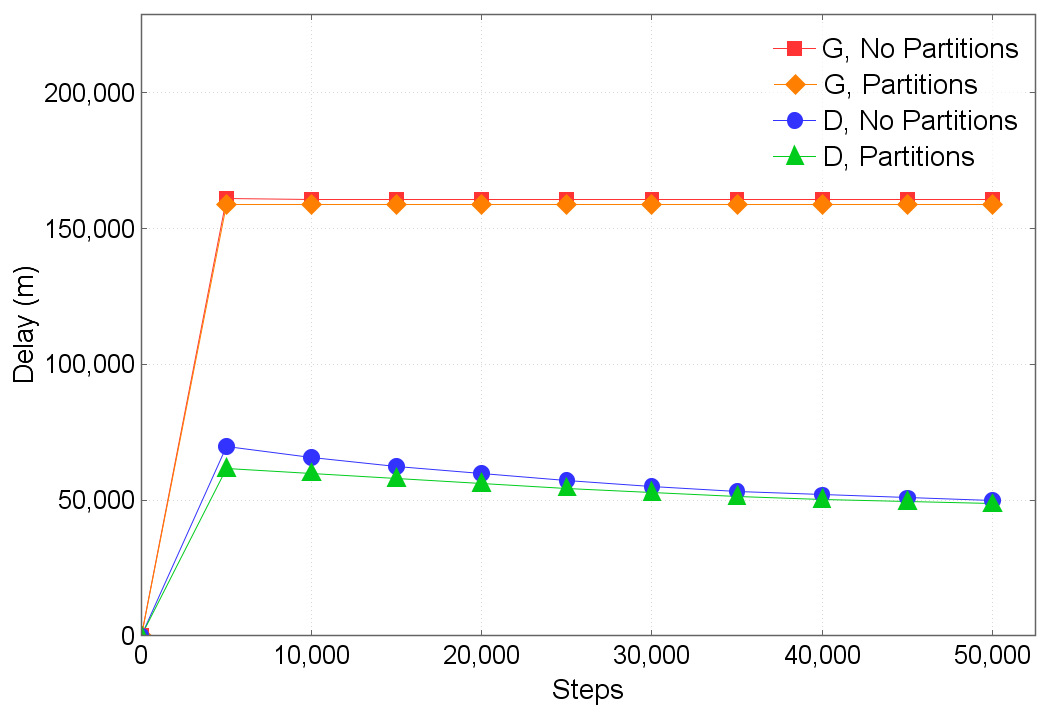
\includegraphics[width=1.0\columnwidth]{ClusterVsNoClusterNonGreedy-Delay}
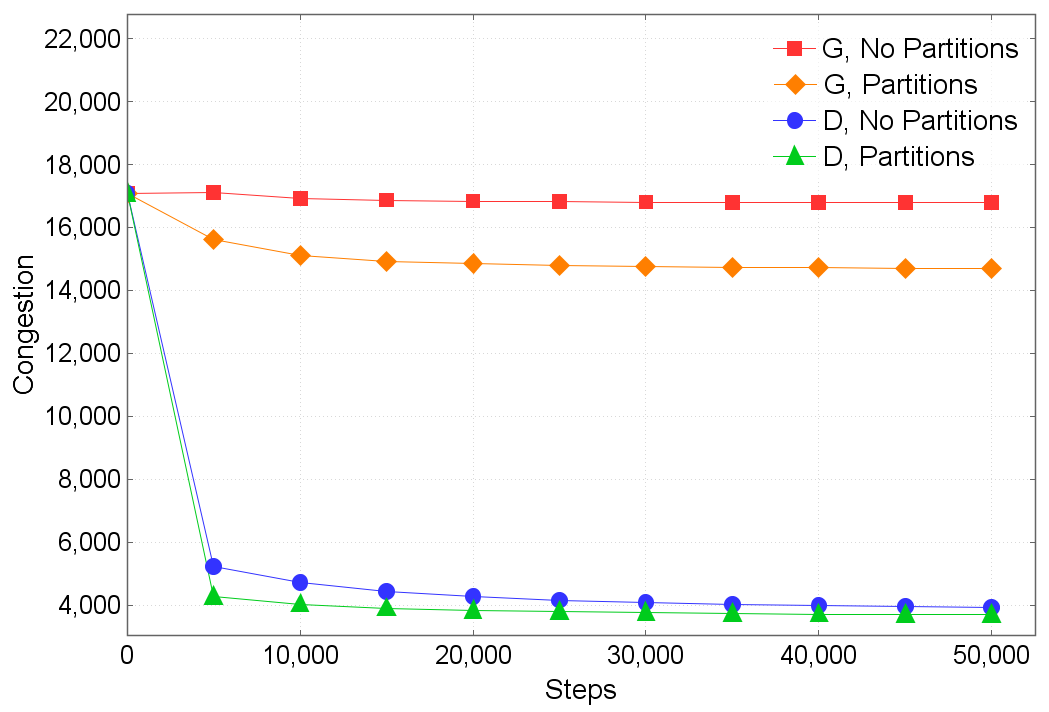
\includegraphics[width=1.0\columnwidth]{ClusterVsNoClusterNonGreedy}
\caption{Using the system-level performance as a evaluation does not work well in this large agent system. The difference evaluation was able to lower congestion much more, but could not manage to also reduce delay.}
\label{NonClusterVsCluster}
\end{figure}

Figure \ref{NonClusterVsCluster} shows that the system-level evaluation performs better using partitions. When looking closer at congestion and delay, we find that using the system-level evaluation did not improve delay at all, and only improved congestion slightly. There is too much noise caused by other agents within this system for the system-level evaluation to be a good evaluation. With the partitions, the noise was greatly reduced and therefore agents were given a better evaluation. The difference evaluation on the other hand is able to more easily capture an agents impact on congestion, and dramatically reduced congestion. The difference evaluation also benefits much less from the partitioning than the system-level evaluation. This is because the difference evaluation is able to reduce the signal-to-noise within the learning signal on its own, while the system-level evaluation requires the partitioning to attempt to accomplish the same reduction. The partitioning benefits the difference evaluation time complexity, rather than pure performance.

This is a fine solution if some congestion was allowed in the system, as both delay and congestion are greatly decreased. In our problem however, we would like to reduce congestion down to zero. This is only possible with the greedy scheduler.

\subsection{Learning with Hard Constraints}
By adding the greedy scheduler we were able to eliminate congestion by sacrificing delay. Some aircraft in normally highly-congested areas are forced to delay many hours, while most aircraft don't need to delay at all. Although high, this delay is required to guarantee a safe environment for all aircraft. 

This is a difficult scheduling problem that has a very specific solution. Although the greedy scheduler is suboptimal, it performs well in this domain without the use of agents. Most planes do not need to be delayed, and the ones that do can simply be delayed until no congestion occurs. This solution does not take into account any interactions between aircraft, and cannot perform the coordination required to reduce delay even further. Our approach finds a better solution by finding these subtle coordination situations and taking advantage of them.  

Figure \ref{ClusterRewardsGreedyG} shows that although using partitions are an improvement, using our system-level evaluation still does not minimize delay more than the simple greedy solution. This fitness evaluation function does not give the agents an accurate enough fitness to discover the subtle coordination improvements, and additionally takes a very long time to converge to a suboptimal solution. 

\begin{figure}[tbh!]
\centering
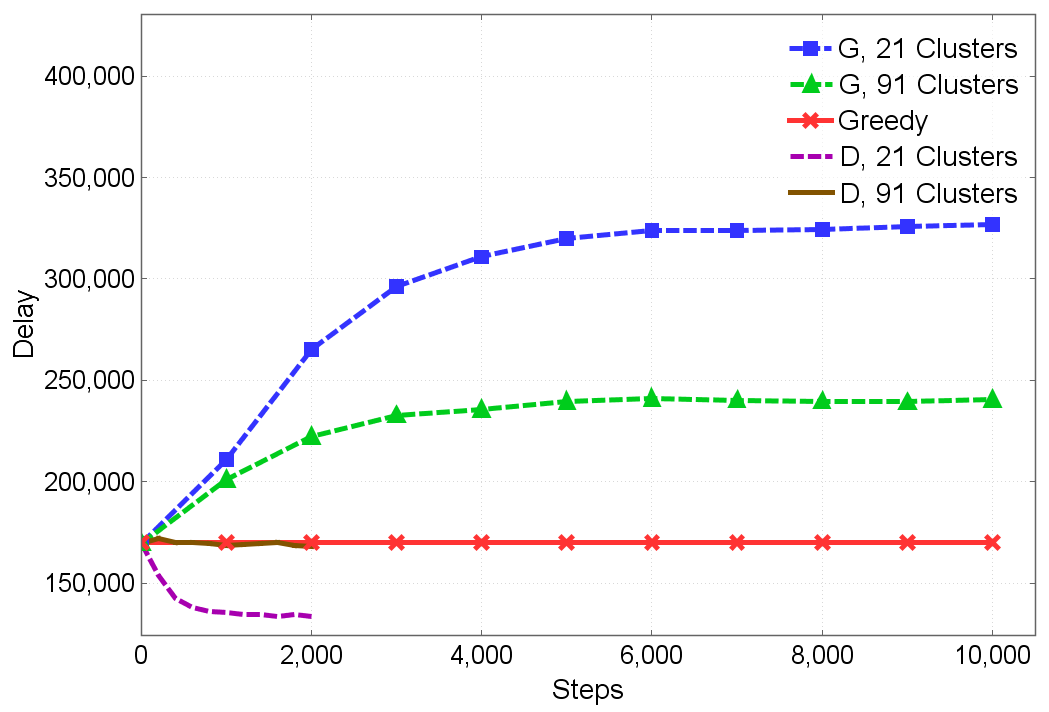
\includegraphics[width=1.0\columnwidth]{ClusterRewardsGreedyGEvo}
\caption{The highest and lowest level of partitioning for the difference evaluation (D) and system-level evaluation (G) is displayed here. The difference evaluation performed better using a smaller number of partitions, where the system-level evaluation performed worse. Using this learning approach, the system-level evaluation performance could never become better than the greedy scheduler. Note: The performance of D, 91 Clusters is very close to the greedy performance. A closer look at the difference evaluation results are in Figure 5.}
\label{ClusterRewardsGreedyG}
\end{figure}

The difference evaluation was able to communicate to the population members a fitness that is more representative of their contribution to team performance. This reduced the the signal-to-noise ratio in fitness evaluations and greatly assists the agents in choosing the optimal action. This accurate evaluation allows agents to quickly find the subtle actions that will allow them to easily coordinate with other agents, thereby quickly reducing the delay past the greedy scheduling solution. 

As mentioned earlier, the greedy scheduler gives a good, but not optimal scheduling policy. This leads us to use the greedy scheduling policy as a good place to start searching. Bootstrapping each agent to choose zero delay reduces the overall amount of computation time needed to compute the difference evaluation by giving the agents a good policy from the start. Agents can then explore other actions with a frequency based on the mutation rate and can discover potentially better actions.

Figure \ref{ClusterRewardsGreedyG} shows the best-performing simulation using the system-level evaluation involved the highest number of partitions, while the best performing simulation using the difference evaluation used the lowest number of partitions. This agrees with the results in section 4.1. As the number of agents per partition increased, more agents affect the fitness. The system-level evaluation has no way for an agent to filter out the noise of other agents, thus receiving noisy feedback, and therefore benefits more from a larger number of partitions. The difference evaluation on the other hand removes the noise out of the system-level evaluation and agents can therefore coordinate in the larger partitions easier.

\begin{figure}[tbh!]
\centering
\includegraphics[width=1.0\columnwidth]{greedyVsDifferenceEvo}
\caption{A closer look at the difference evaluation performance using the smaller number of partitions shows a 21\% improvement over the greedy scheduling solution. Note that errors bars are not included. Over 10 statistical runs the standard deviation was negligible. }
\label{greedyVsDifferenceEvo}
\end{figure}

Although it would result in the best performance, using the difference evaluation with the greedy scheduler is an impossible task. With 35,000 aircraft in the system, one evaluation step takes 3 hours due to the rescheduling needed at every difference calculation. Agent partitions allowed us to greatly speed up this number, as only agents within a partition need to be rescheduled during the difference calculation. Figure 5 shows the magnitude of performance gain when using the difference evaluation and partitioning, while Table 1 shows that the speedup of using different partition sizes is significant, but has a high cost to performance. Since partitions had some overlap, actions in one partition may affect the agents in another partition, meaning that the higher the number of partitions the less information the agents receive in the difference evaluation. Larger partitions end up leading to better overall performance at the cost of computation time.

\subsection{Partition Comparisons for Hard Constraints}
Speed and performance of partitions were negatively correlated. As the number of partitions were reduced, the greedy scheduler was required to schedule more planes per difference calculation. This greatly increased the amount of time per evaluation step. Additionally, with a smaller number of partitions, planes that slightly affected each other were partitions together. This allowed higher quality evolution since a population member's fitness encompassed the effects of basically all of the other agents that impact it. 

This speed and performance correlation also occurs within the same partition. As the delay decreases, more agents switch from taking the zero delay action to taking a more intelligent action allowing better scheduling. This means that the agent no longer equals the counterfactual, and the difference evaluation calculation cannot be skipped. Table 1 shows this in more detail. This table compares the amount of time taken per evaluation step to the final performance. With the smaller number of partitions, the initial evaluation steps are slower than the final evaluation steps, but the performance is very good. With the large number of partitions, the initial evaluation steps are only slightly less time intensive than the final evaluation steps, leading to very fast simulation times, but result in a worse final performance. This is an artifact of the agents coordinating and finding a more optimal action than picking zero delay.

\begin{table}[tbh!]
\begin{tabular}{|l|c|c|c|c|c|}
\hline
& \multicolumn{3}{|c|}{Time per run} & &Final Delay\\
Partitions & \multicolumn{3}{|c|}{seconds} &Steps&in\\
&First&Avg&Last&&minutes\\
\hline
Greedy & 5 & 5 & 5 & * & 169,750 \\
\hline
1 & 3hr & * & * & * &* \\
\hline
21 & 116 & 364 & 402 & 2,000 & 134,050\\
\hline
24 & 64.8 & 155 & 173 & 2,000 & 139,630\\
\hline
29 & 37.1 & 89.2 & 100.2 & 2,000 & 145,630\\
\hline
38 & 23.3 & 46.9 & 52.38 & 2,000 & 154,770\\
\hline
56 & 16.6 & 26.6 & 29.2 & 2,000 & 162,710\\
\hline
91 & 13.5 & 20.3 & 22.6 & 2,000 & 167,990\\
\hline
\end{tabular}
\caption{With the greater number of partitions, the performance decreases and speed increases. Various partition numbers allow the ability to choose between final performance and speed performance. Note that data for one partition, the entire D calculation, cannot realistically be evaluated and is shown here for comparison purposes.}
\label{TimingTable}
\end{table}

The agent partitioning allows applications to become very situation dependent. If results need to be found very quickly, a larger number of partitions could be used, and this approach will find a policy still better than using the greedy scheduler. On the other hand if time spent is not important, the smaller number of partitions will result in a very good policy 21\% better than the greedy scheduler. 

\section{Conclusion and Future Work}
The main contribution of this paper is to present a distributed adaptive air traffic flow management algorithm with implementable results. The method introduced is based on agents representing airport gates within the NAS choosing aircraft ground delay with the intent of minimizing delay within the system. It uses CCEAs in combination with the difference evaluation and hard constraints on congestion. This is typically an impossible problem, but we introduce agent partitions to dramatically reduce the time complexity by up to 30x per evaluation step, leading to a 21\% increase in performance over the greedy solution. The different sized partitions also allowed the implementation to be dynamic to the situation. If results need to be computed quickly, a large number of partitions could be used, where a smaller number of partitions could be used if performance was more important than speed. The ease of adding simple ground delays in combination with the large increase in performance over currently used approaches makes this approach easily deployable and effective.

Future work in the ATFMP would mainly involve increasing both performance and speed. Speed could easily be improved through the use of parallel computing and optimization the greedy scheduler. Approaches improving team based coordination such as leniency \cite{Panait} and coordination graphs \cite{Kok:2006:CMR:1248547.1248612,Coordination} could be additional ways to increase performance at the cost of speed. Further analysis will be done to attempt to add these coordination methods to this approach while minimizing the cost to speed. Additional improvements in speed involve a more advanced greedy scheduler and better partitioning techniques.

Further advances in the simulator could be easily worked into the problem. Attributes such as flight importance or unscheduled delays, such as weather or maintenance, could be easy implemented. Additionally, a level of uncertainty can be added to analyze how robust this particular solution is to unknown changes. This approach may be dynamic enough to be robust to all of these changes, and this is a subject of further research.

\bibliography{references}{}
\bibliographystyle{plain}


\end{document}
